\section{Исследование и построение решения задачи}
\label{sec:research_and_solving} \index{research_and_solving}
\subsection{Описание предложенного решения задачи}
В этом разделе будет описаны методы построения представления сложноструктурированных событий, рассмотрена интерпретируемость каждого из представлений, и показано, какие методы можно использовать для решения  непосредственно задачи прогнозирования.

Схема предложенного подхода к решению поставленной задачи показана на Рис. \ref{fig:framework_structure}, далее в этой секции будут детально описаны все компоненты предложенного подхода.

\begin{figure}
    \centering
    \includegraphics[width=\linewidth]{images/framework_scheme.png}
    \caption{Структура предложенного подхода}
    \label{fig:framework_structure}
\end{figure}

\subsubsection{Построение представления событий}
\label{subsub:repr}
% PCA
% NMF Неотрицательная факторизация матрицы
% AE Нейросетевой автокодировщик
При построении представления сложноструктурированных событий и с учетом их временной неравномерности,
мы требуем от такого представления возможность агрегации по времени. Также для неявного (скрытого) представления событий хотелось бы иметь возможность его интерпретации, чтобы можно было производить какой-то анализ как самого представления, так и использующих его моделей.

Перед переходом к построению представления, опишем предлагаемые методы обработки различных типов признаков.
Числовые и бинарные признаки не предобрабатывались, категориальные признаки переводились в бинарные с помощью унитарного кодирования (one-hot encoding). Для категориальных признаков также можно использовать любой метод перевода их в бинарные/числовые признаки: кодирование уникальными значениями и другие.
Текстовые описания можно преобразовать в числовые вектора одним из многих способов: латентным размещение Дирихле (LDA), кодированием tf-idf или нейросетевыми моделями (word2vec, doc2vec, скрытое представление с помощью LSTM). В этой работе я использовал латентное размещение Дирихле для предобработки текстовых данных. После такой обработки все признаки становятся либо числовыми, либо бинарными.

Несмотря на то, что числовые и бинарные признаки обладают возможностью агрегации по времени, велика вероятность того, что они избыточны, а значит можно найти такое представление, которое переведет исходные признаки в пространство меньшей размерности и будет более уместно для использования в задаче прогнозирования. 

В качестве базового подхода были рассмотрены такие методы понижения размерности как Метод главных компонент (PCA \cite{pca_orig}), Неотрицательная факторизация матриц (NMF \cite{nmf_orig}). В этой работе было решено остановиться на более тщательном исследовании применимости неотрицательной факторизации матриц. 

Общая идея факторизации матрицы заключается в следующем: 
Пусть $n$ -- количество событий, $d$ -- размерность вектора признаков каждого события. Обозначим исходную матрицу описывающую события как $V$, $V \in \mathbf{R}^{n \times d}$. Задача факторизация матрицы $V$ заключается в нахождении матриц $W \in \mathbf{R}^{n \times k}, H \in \mathbf{R}^{k \times d}$, $k \ll d$ таких, что эти матрицы $W, H$ минимизируют $||V - W \cdot H||$. Из такого разложения видно, что матрица $H$ показывает соотношение между исходными $n$ признаками и новыми $k$ признаками. Эти новые $k$ признаков мы будем в дальнейшем называть тематиками или скрытыми (латентными) признаками. Также будем называть матрицу $W$ матрицей \textit{событий-тематик}, а матрицу $H$ матрицей \textit{тематик-признаков}. Схема работы этого метода приведена на Рис. \ref{fig:nmf_scheme}
\begin{figure}
\centering
  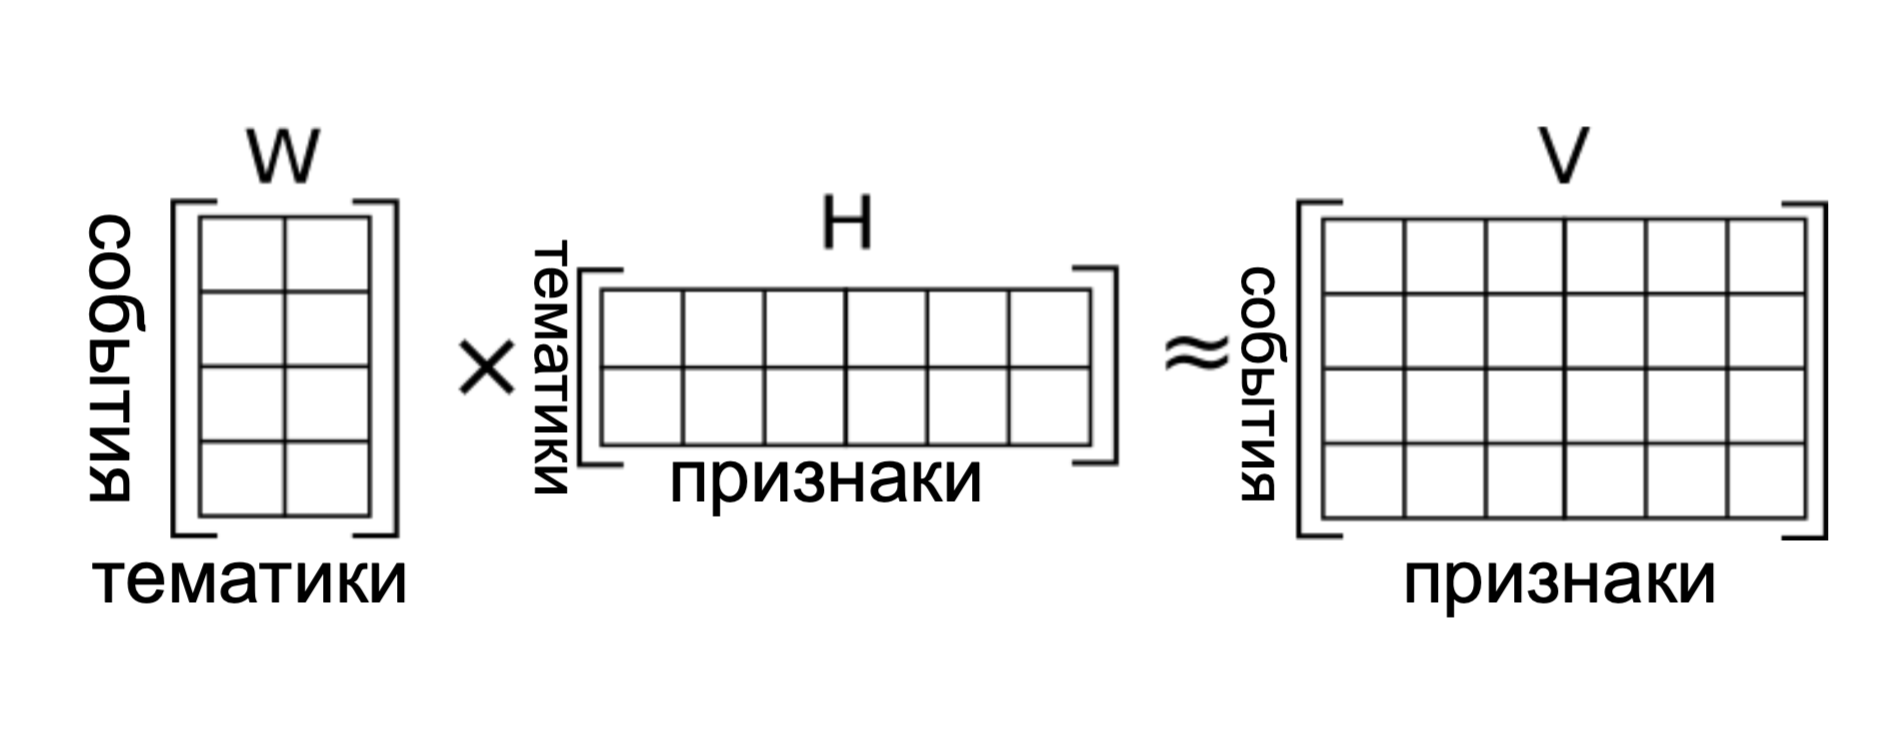
\includegraphics[width=.9\linewidth]{images/nmf_scheme.png}
  \caption{Схематическое изображение работы алгоритма NMF}
  \label{fig:ae_arch}
\end{figure}
При использовании неотрицательной факторизации матрицы, тематики представляют из себя линейные комбинации исходных признаков с неотрицательными весами, что делает интерпретируемость этих тематик тривиальной задачей.

Процесс факторизации является итеративным, в начале матрицы $W, H$ инициализируются неотрицательными значениями, затем они поочередно обновляются следующим образом:
$$H^{n+1}_{[i,j]} = H^n_{[i,j]} \frac{((W_n)^TV)_{[i,j]}}{((W^n)^TW^nH^n)_{i,j]}}$$
$$W^{n+1}_{[i,j]} = W^n_{[i,j]} \frac{(V(H^{n+1})^T)_{[i,j]}}{(W^nH^{n+1}(H^{n+1})^T)_{[i,j]}}$$

После того, как процесс сойдется, мы получаем матрицы $W,H$.

В качестве более продвинутого метода построения представления событий будет рассмотрен глубокий нейросетевой автокодировщик (далее -- просто автокодировщик) \cite{ae_orig}. 
Автокодировщик это специальная архитектура искусственных нейронных сетей, позволяющая применять обучение без учителя при использовании метода обратного распространения ошибки.

Простейшая архитектура автокодировщика — сеть прямого распространения, схожая с многослойным перцептроном и содержащая блок слоев для перевода входного вектора в скрытый код (кодировщик) и блок слоев для перевода скрытого кода в выходной вектор (декодировщик). В отличие от стандартных нейросетевых архитектур, выходной слой автокодировщика содержит столько же нейронов, сколько и входной слой, а задачей всей сети является перевод входного вектора в код меньшей размерности (кодировщик) и дальнейшее восстановление вектора из его кода с минимизацией ошибки восстановления (декодировщик). Пример архитектуры однослойного автокодировщика представлен на Рис. \ref{fig:ae_arch}.
\begin{figure}
\centering
  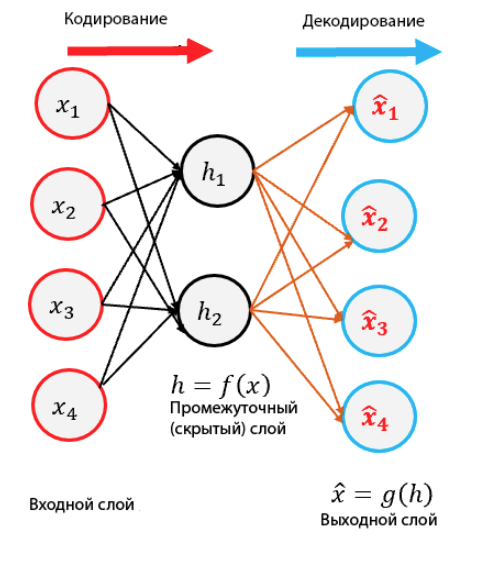
\includegraphics[width=.5\linewidth]{ae_arch_ru.png}
  \caption{Пример архитектуры простого автокодировщика}
  \label{fig:ae_arch}
\end{figure}

Более формально, автокодировщик нелинейно преобразует входной вектор $x \in \mathbf{R}^d$ в $z \in \mathbf{R}^k$, а затем производит реконструкцию вектора $x$ используя $z$. В результате реконструкции получается вектор $x' \in \mathbf{R}^d$, и задача автокодировщика -- минимизировать ошибку восстановления $L(x,x')$ (например $L(x,x')=||x - x'||$).

После обучения модели с такой архитектурой, можно использовать только ее первую часть (кодировщик) для получения $z^*$ их произвольного входного вектора $x^*$ и использовать этот код $z^*$ как скрытое представление события. В таком случае скрытыми тематиками будем называть элементы вектора $z^*$.
Так как преобразования кодировщика нелинейны, интерпретация скрытого кода затруднительна, эта проблема будет рассмотрена отдельно в следующем разделе.

% Auxiliary features
В процессе исследования решения задачи, было решено добавить два дополнительных признака для выделения более явной регрессионной компоненты. Для каждого агрегационного периода вычислялось:
\begin{enumerate}
   \item $N_{all}$, общее количество событий, входящих в этот период
   \item $N_{target}$, количество целевых событий, входящих в этот период
\end{enumerate}

Эти признаки можно было бы назвать ''экспертными'' или ''созданными вручную'', но они не умаляют общности подхода, так как применимы для задачи прогнозирования событий в целом.

% Recon features
Также вместе с признаками, полученными с помощью автокодировщика было предложено использовать в качестве дополнительного признака ошибку восстановления автокодировщика (т.е. признак, показывающий, насколько восстановленный автокодировщиком вектор признаков отличается от исходного вектора признаков):

$recon\_err = x' - x$, следуя нотации введенной ранее.

Мотивация добавления подобного признака следует из области выявления аномалий \cite{anomaly_detection_ae} и заключается в следующем: если исходный вектор признаков сильно отличается от восстановленного вектора признаков (большая ошибка восстановления), то есть основания полагать, что этот вектор является в некотором смысле аномальным и модель с помощью значения такого признака сможет учитывать аномальность конкретного события.

\subsubsection{Интерпретируемость представления}
\label{subsub:interp}
Как было сказано выше, важной характеристикой скрытого представления событий является его интерпретируемость. Если у представления такое свойство есть, то становится возможным анализ полученных тематик, а так же анализ результатов прогнозирования и их более глубокое понимание.

По своей природе скрытые признаки, выделенные неотрицательной факторизацией матриц и методом главных компонент интерпретируемы, поскольку эти скрытые признаки представляют собой линейные комбинации исходных признаков. В случае неотрицательной факторизацией матриц, если рассмотреть вышеупомянутую матрицу \textit{тематик-признаков}, можно увидеть, что каждая тематика описывается набором неотрицательных весов, соответствующих оригинальным признакам. Чем больше вес у некоторого признака, тем более сильный вклад этот признак вносит в данную тематику. 
Пример того, как можно описать одну из тематик, выделенных NMF, можно увидеть на Рис. \ref{fig:nmf_topic}. На этом рисунке изображены 9 исходных признаков с наибольшими весами, т.е. вносящих максимальный вклад в тематику.
\begin{figure}
  \centering
  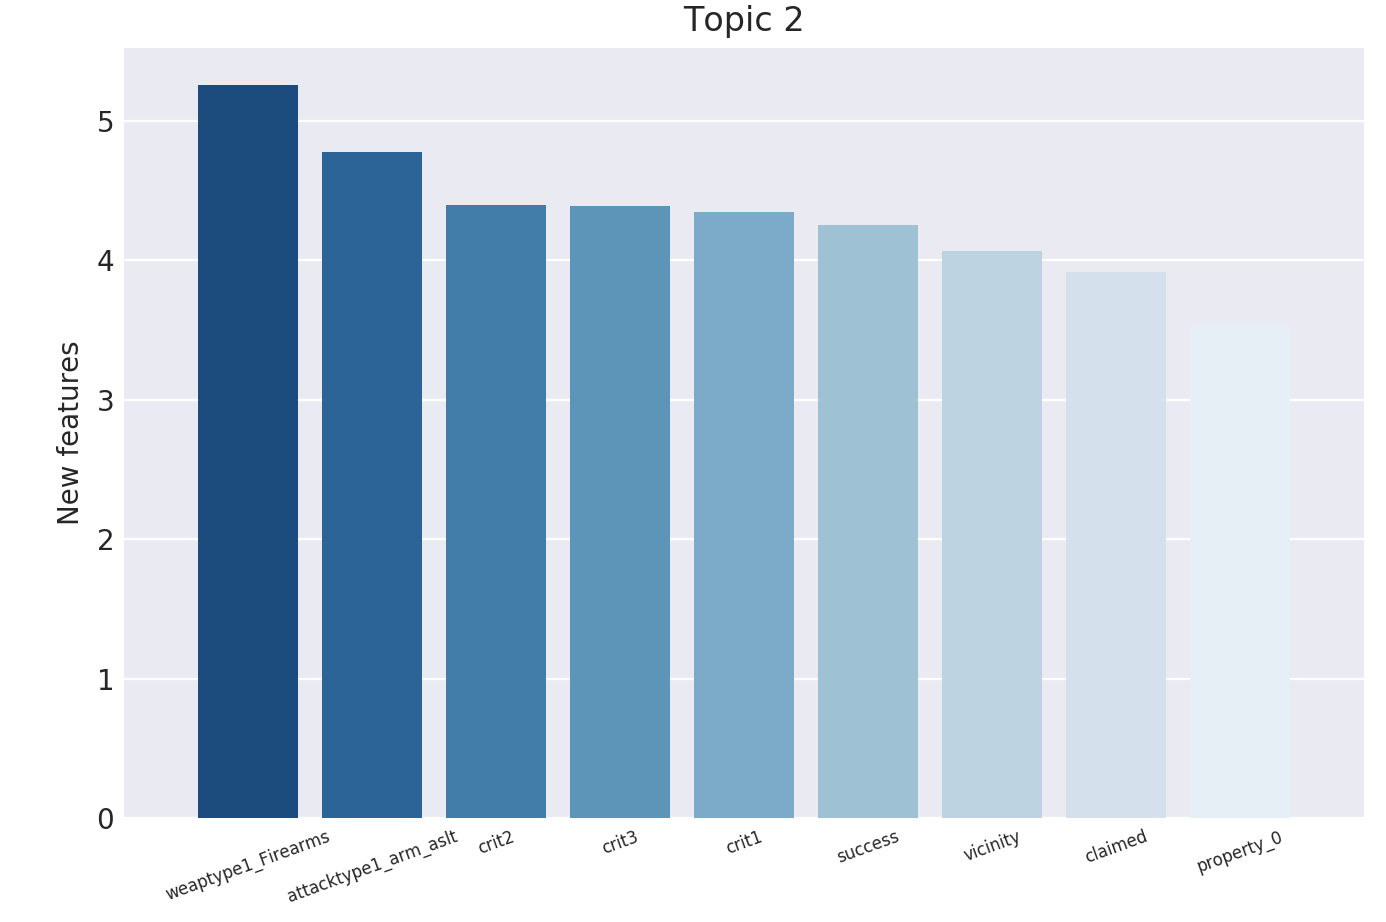
\includegraphics[width=.8\linewidth]{nmftopic.png}
  \caption{Пример интерпретации тематики, выделенной с помощью неотрицательной факторизации матриц}
  \label{fig:nmf_topic}
\end{figure}

В случае, когда преобразование исходного пространства признаков более сложное и нелинейное, необходимы другие методы интерпретации.
В данной работе предлагается метод, основанный на текстовых описаниях, доступных хотя бы для части событий.

Первый шаг получения интерпретации тематик это извлечь все доступные текстовые описания, обработать их стандартными методами (привести к нижнему регистру, убрать пунктуацию и стоп-слова, нормализовать формы слов) и составить словарь $W$ из полученного набора термов. Обозначим размер этого словаря как $|W|$.

Затем выберем из всего множества событий те, у которых есть текстовые описания, и каждому событию сопоставим $|W|$ бинарных признаков, показывающих вхождение или отсутствие каждого слова из словаря в текстовом описании этого события.

После составления таких признаков необходимо найти значение $v_{i,j}$ для $i$-й тематики $T_i$ и $j$-го бинарного признака  $B_j$, соответствующего $j$-му ключевому слову. Значение $v_{i,j}$ считается по всем выбранным событиям следующим образом:  

$$
v_{i,j} = \frac{r_{i,j}}{\max\limits_{k \neq i} r_{k,j}}\mbox{, где }
r_{i,j} = 1 - \mbox{corr}(T_i, B_j)^2,$$ и оно обратно пропорционально тому, насколько $j$-е ключевое слово ''важно'' для описания $i$-й тематики. Выбирая для каждой из тематик $K$ ключевых слов с максимальными значениями $v$, мы получаем текстовые описания (т.е. способ интерпретации) этих тематик.
Как показали эксперименты, даже менее чем 20\% событий с текстовыми описаниями достаточно для построения описаний тематик. Подробный алгоритм получения текстовых описаний для тематик описан в блоке Алг. \ref{alg:kw_interp}.


\begin{algorithm}
    \caption{Алгоритм интерпретации тематик}\label{alg:kw_interp}
    \begin{algorithmic}
    \STATE \textbf{Входные данные.} Матрица значений скрытых тематик для каждого события $T = \{t_{i,j}\}, \in \mathbf{R}^{k \times n}$, текстовые описания событий $d'_j$, требуемое количество слов в текстовом описании каждой из тематик $K$
    \STATE \textbf{Результат.} набор из $K$ ключевых слов для каждой тематики $\theta_i,\ i=1..k$
    \STATE инициализация: $\theta_i = \varnothing,\ i=1..k$;
    \FOR{$j=1$ \TO $n$}
        \STATE $d_j \gets \mbox{предобработать}(d'_j)$;
        \STATE $kw_j \gets \mbox{извлечь\_ключевые\_слова}(d_j)$;
    \ENDFOR
    \item $W \gets \bigcup\limits_{j=1}^n kw_j, \ W=\{w_i\}$;
    \item $B \gets \{b_{i,j}\},\ b_{i,j} = \mathbf{I}_{w_i \in d_j},\ B \in \mathbf{R}^{|W| \times n}$;
    \FOR{$i = 1$ \TO $k$}
        \FOR{$j = 1$ \TO $|W|$}
            \STATE $r_{i,j} \gets 1 - \mbox{corr}(T_i, B_j)^2$;
            \STATE $v_{i,j} \gets \frac{r_{i,j}}{\max\limits_{k \neq i} r_{k,j}}$;
        \ENDFOR
    \ENDFOR
    \FOR{$k = 1$ \TO $K$}
        \STATE $j=\argmin\limits_{\{j: w_j \notin \theta_i\}} v_{i,j}$\;
        \STATE $\theta_i \gets$ add $w_j$\;
    \ENDFOR
    \end{algorithmic}
\end{algorithm}


Как дополнительный результат этого метода, можно получить описание любого события ключевыми словами, выбрав некоторое количество ключевых слов из описаний каждой тематики пропорционально значениям этих тематик у события.

\subsubsection{Прогнозирование событий}
% % classic: RF, LR, MachineLearning \subsubsectionЛогистическая/линейная регрессия (LogReg/LinReg)
% % NN: Модель с долгой краткосрочной памятью (LSTM}
\label{subsub:forecasting}
После того как получено подходящее представление событий, возникает вопрос об их прогнозировании. Для использования классических и хорошо изученных методов необходимо каждому событию сопоставить бинарную метку -- является ли оно интересующим нас событием.
Обозначим множество всех событий как  $E_{all}$, а множество интересующих нас событий как $E_{in}$. Тогда метка $y_e$ для события $e$ определяется следующим образом: $1$ если $e \in E_{in}$ и $0$ иначе.

В дальнейших рассуждениях будем подразумевать, что каждое событие $e$ имеет временную метку $t_e$ и набор значений тематик $x_e$ (т.е. представление события $e$, описывающее это событие).

После выбора размера интервала агрегации $\Delta t$, мы получаем разбиение временной шкалы на интервалы размера $\Delta t$. 
Для каждого такого интервала $T_i$ мы получаем усредненные значения тематик событий, принадлежащих этому интервалу.
$$\bar{x_i} = \frac{1}{|\{i: t_{e_i} \in T_i\}|} \sum_{\{i: t_{e_i} \in T_i\}}{x_{e_i}}$$ 

Агрегация меток событий производится в зависимости от решаемой задачи:
$$\bar{y_i} = \sum_{\{i: t_{e_i} \in T_i\}}{y_{e_i}},$$ для прогнозирования количества событий и

$$\bar{y_i} = max_{\{i: t_{e_i} \in T_i\}}{y_{e_i}}, $$ для прогнозирования вероятности события.

После выполнения указанных выше преобразований, мы получаем многомерный временной ряд, где значения $\bar{x}_{0,1,...}$ являются значениями этого ряда. 
Поскольку прогнозирование будет основываться на исторических данных, обозначим количество используемых предшествующих интервалов за $L$. С учетом этих обозначений, формально проблему прогнозирования можно описать как нахождение $\hat{y}_{i+1}$ при данных $\bar{x}_{i-L+1}, \bar{x}_{i-L+2}, ...,\bar{x}_{i}$, где $\hat{y}_{i+1}$ это предсказанное значение $\bar{y}_{i+1}$.

В данной работе предлагаются два различных подхода к такому прогнозированию. Первый и базовый подход -- объединить значения тематик с $L$ предшествующих интервалов в один вектор, опционально добавить дополнительные признаки предложенные выше и используя классические методы обучить на этих данных классификатор или регрессор, в зависимости от задачи.

Вторым подходом является использование нейросетевой архитектуры долгой краткосрочной памяти (Long short-term memory; LSTM) \cite{lstm_orig} .

Архитектура искусственных нейронных сетей LSTM основана на идее рекуррентных нейронных сетей (RNN). Рекуррентные нейронный сети -- семейство нейронных сетей, в которых связи между узлами формируют направленную последовательность. Также у рекуррентных нейронных сетей есть внутреннее состояние  (память), с помощью которого такие сети могут работать с входными последовательностями различной длины. Основной недостаток данной архитектуры -- проблемы с градиентами при работе алгоритма обратного распространения ошибки по времени (т.е. по элементам последовательности в обратном порядке). В случае, если последовательность достаточно длинная, может возникнуть проблема исчезающих градиентов, при которой градиенты из-за очень долгого пути и большого числа умножений на матрицы вырождаются в 0 и веса нейронной сети перестают обновляться. Другая и прямо противоположная проблема -- проблема зашкаливания градиентов, при которой, опять же из-за длинного пути градиентов и большого количества умножений градиенты неконтролируемо и очень быстро растут, стремительно превышая разумные пределы. Нейросетевая архитектура долгой краткосрочной памяти призвана решить обе эти проблемы, в ней на каждой итерации (т.е. при обработке каждого нового элемента последовательности) происходит не просто умножение входных данных на матрицу, а обработка этих данных более сложным блоком. Блок содержит в себе \textit{ячейку памяти} и 3 \textit{вентиля}: \textit{входной вентиль}, \textit{выходной вентиль} и \textit{вентиль забывания}. 

Ячейка памяти в сетях долгой краткосрочной памяти интуитивно позволяет запоминать информацию о зависимостях между элементами последовательности. Входной вентиль контролирует то, какая часть входных данных (нового элемента последовательности) будет учитываться при дальнейших вычислениях в блоке. Выходной вентиль контролирует, какая часть информации из ячейки памяти будет использована для вычислений выходного сигнала блока. Вентиль забывания определяет, какая часть данных из памяти сохранится при переходе на следующий шаг, а какая часть будет удалена (забыта). Ключевой особенностью этой архитектуры является то, что благодаря ячейке памяти и структуре блока градиент не исчезает при использовании метода обратного распространения ошибки во времени. Иллюстрация архитектуры блока показана на рис. \ref{fig:lstm_arch}, а вычисления внутри блока производятся следующим образом:\\
$f_t = \sigma_g(W_{f} x_t + U_{f} h_{t-1} + b_f)$ \\
$i_t = \sigma_g(W_{i} x_t + U_{i} h_{t-1} + b_i)$ \\
$o_t = \sigma_g(W_{o} x_t + U_{o} h_{t-1} + b_o)$ \\
$c_t = f_t \circ c_{t-1} + i_t \circ \sigma_c(W_{c} x_t + U_{c} h_{t-1} + b_c)$ \\
$h_t = o_t \circ \sigma_h(c_t),$ \\
где \\
$x_{t}x_t$ — входной вектор,\\
$h_{t}$ — выходной вектор,\\
$c_{t}$ — вектор состояний,\\
$W,\ U$ и $b$ — матрицы параметров и вектор,\\
$f_{t},\ i_{t}$ и $o_{t}$ — векторы вентилей:\\
$f_{t}$ — вектор вентиля забывания, вес запоминания старой информации,\\
$i_{t}$ — вектор входного вентиля, вес получения новой информации,\\
$o_{t}$ — вектор выходного вентиля, кандидат на выход.\\
В формулах выше используются следующие функции: \\
$\sigma_{g}$: функция активации на основе сигмоиды.\\
$\sigma_{c}, \sigma_{h}$: функция активации на основе гиперболического тангенса.\\
$\circ$: произведение Адамара или покомпонентное произведение.

\begin{figure}
  \centering
  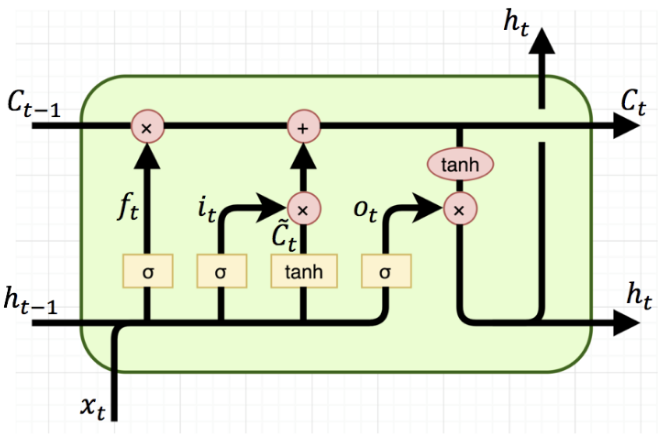
\includegraphics[width=.75\linewidth]{images/lstm_arch.png}
  \caption{Архитектура блока LSTM. $f_t,\ i_t,\ o_t$ - вентили забывания, входа и выхода. $x_t$ -- входной сигнал, $h_t$ -- выходной сигнал и внутреннее состояние блока. $C_t,\ C_{t-1}$ -- состояния ячейки памяти на $t$-м и $t-1$-м шагах соответственно}
  \label{fig:lstm_arch}
\end{figure}


В случае использования сети долгой краткосрочной памяти $L$ векторов будут последовательно поданы на вход модели, начиная с  $\bar{x}_{i-L+1}$ и заканчивая $\bar{x}_{i}$, а на выходе модель будет выдавать прогноз $\hat{y}_{i+1}$. При обучении модель будет пытаться обеспечить на последнем слое такой вывод $\hat{y}_{i+1}$, который был бы максимально похож на прогнозируемое значение $\bar{y}_{i+1}$.

При решении задачи классификации для оценки результатов была использована такая метрика как площадь под ROC-кривой (Area Under Curve, ROC AUC). Главным преимуществом этой метрики является её инвариантность относительно баланса классов. Так, например, при балансе классов 1:9 (на 1 объект из ''положительного'' класса приходится 9 объектов из ''отрицательного класса'') метрика "точность", представляющая из себя долю правильно классифицированных примеров, будет нерепрезентативной: можно получить точность равную 90\% просто предсказывая для всех классов метку ''отрицательный''. При этом, правильно предсказанные 80\% объектов из положительного класса и 80\% правильных предсказаний для негативного класса выглядят как более желаемый результат, но позволяют достичь лишь точности в 80\%.

Поскольку, как известно, в задаче классификации предсказания модели лежат в интервале $[0, 1]$, принадлежность объекта к положительному или отрицательному классу ($y' \in \{1, -1\}$) зависят от коэффициента принадлежности к положительному классу $p$, предсказанного моделью, и выбранного порога $\omega_0$:
$$
y' =    \begin{cases}
			1, & p >= \omega_0\\
            -1, & p < \omega_0
	    \end{cases}
$$

Для вычисления метрики ROC AUC необходимо ввести понятия доли ложных положительных классификаций (False Positive Rate, FPR) и доли верных положительных классификаций (True Positive Rate, TPR):

$$
FPR(y,y') = \frac{\sum_{i=1}^N [y'_i = +1][y_i = -1]}{\sum_{i=1}^N [y_i = -1]}
$$

$$
TPR(y,y') = \frac{\sum_{i=1}^N [y'_i = +1][y_i = +1]}{\sum_{i=1}^N [y_i = +1]}.
$$

Видно, что значения FPR и TPR зависят от выбранного порога $\omega_0$. ROC-кривая показывает зависимость TPR от FPR при варьировании этого порога. Из ее свойств стоит отметить, что она проходит из точки (0, 0) при $\omega_0 = min_{i=1..N} p_i$ в точку (1, 1) при $\omega_0 = max_{i=1..N} p_i$. Площадь под этой кривой (AUC) представляет из себя агрегированную характеристику качества классификации, и чем больше значение этой площади, тем лучше модель.

В задаче регрессии было решено использовать метрику средней абсолютной нормированной ошибки (Mean absolute scaled error, MASE). Сама метрика представляет из себя значение средней абсолютной ошибки нормированное на величину изменчивости прогнозируемых значений и часто используется при оценке качества прогнозирования временных рядов.

Стоит отметить следующие свойства этой метрики:
\begin{itemize}
    \item Инвариантность к мастштабу значений: поскольку в рамках вычисления метрики производится нормировка на изменчивость прогнозируемых данных, эта метрика может быть использована для сравнения на данных разной величины.
    \item Адекватное поведение при $y \rightarrow 0$: многие другие метрики предполагают деление на истинные значения $y_i$ и таким образом принимают сильно смещенные значения при $y_i \rightarrow 0$. Это особенно заметно при вычислении метрик для таких задач, как прогнозирование температуры, где прогнозируемые значения могут быть разных знаков или часто быть равными 0.
     \item Симметричность: метрика средней абсолютной нормированной ошибки ''штрафует'' одинаково ошибки прогноза как в меньшую, так и в большую сторону.
\end{itemize}

Значение метрики вычисляется по следующей формуле:
$$
MASE(y, y') = \frac{MAE(y, y')}{\frac{1}{N-1}\sum_{i=2}^{N} |y_i - y_{i-1}|},
$$ где 
$$MAE(y, y') = \frac{1}{N}\sum_{i=1}^{N} |y_i - y'_i|$$
Здесь $y$ обозначает истинные метки для периода, а $y'$ - метки, предсказанные моделью.

\begin{figure}[t]
  \centering
  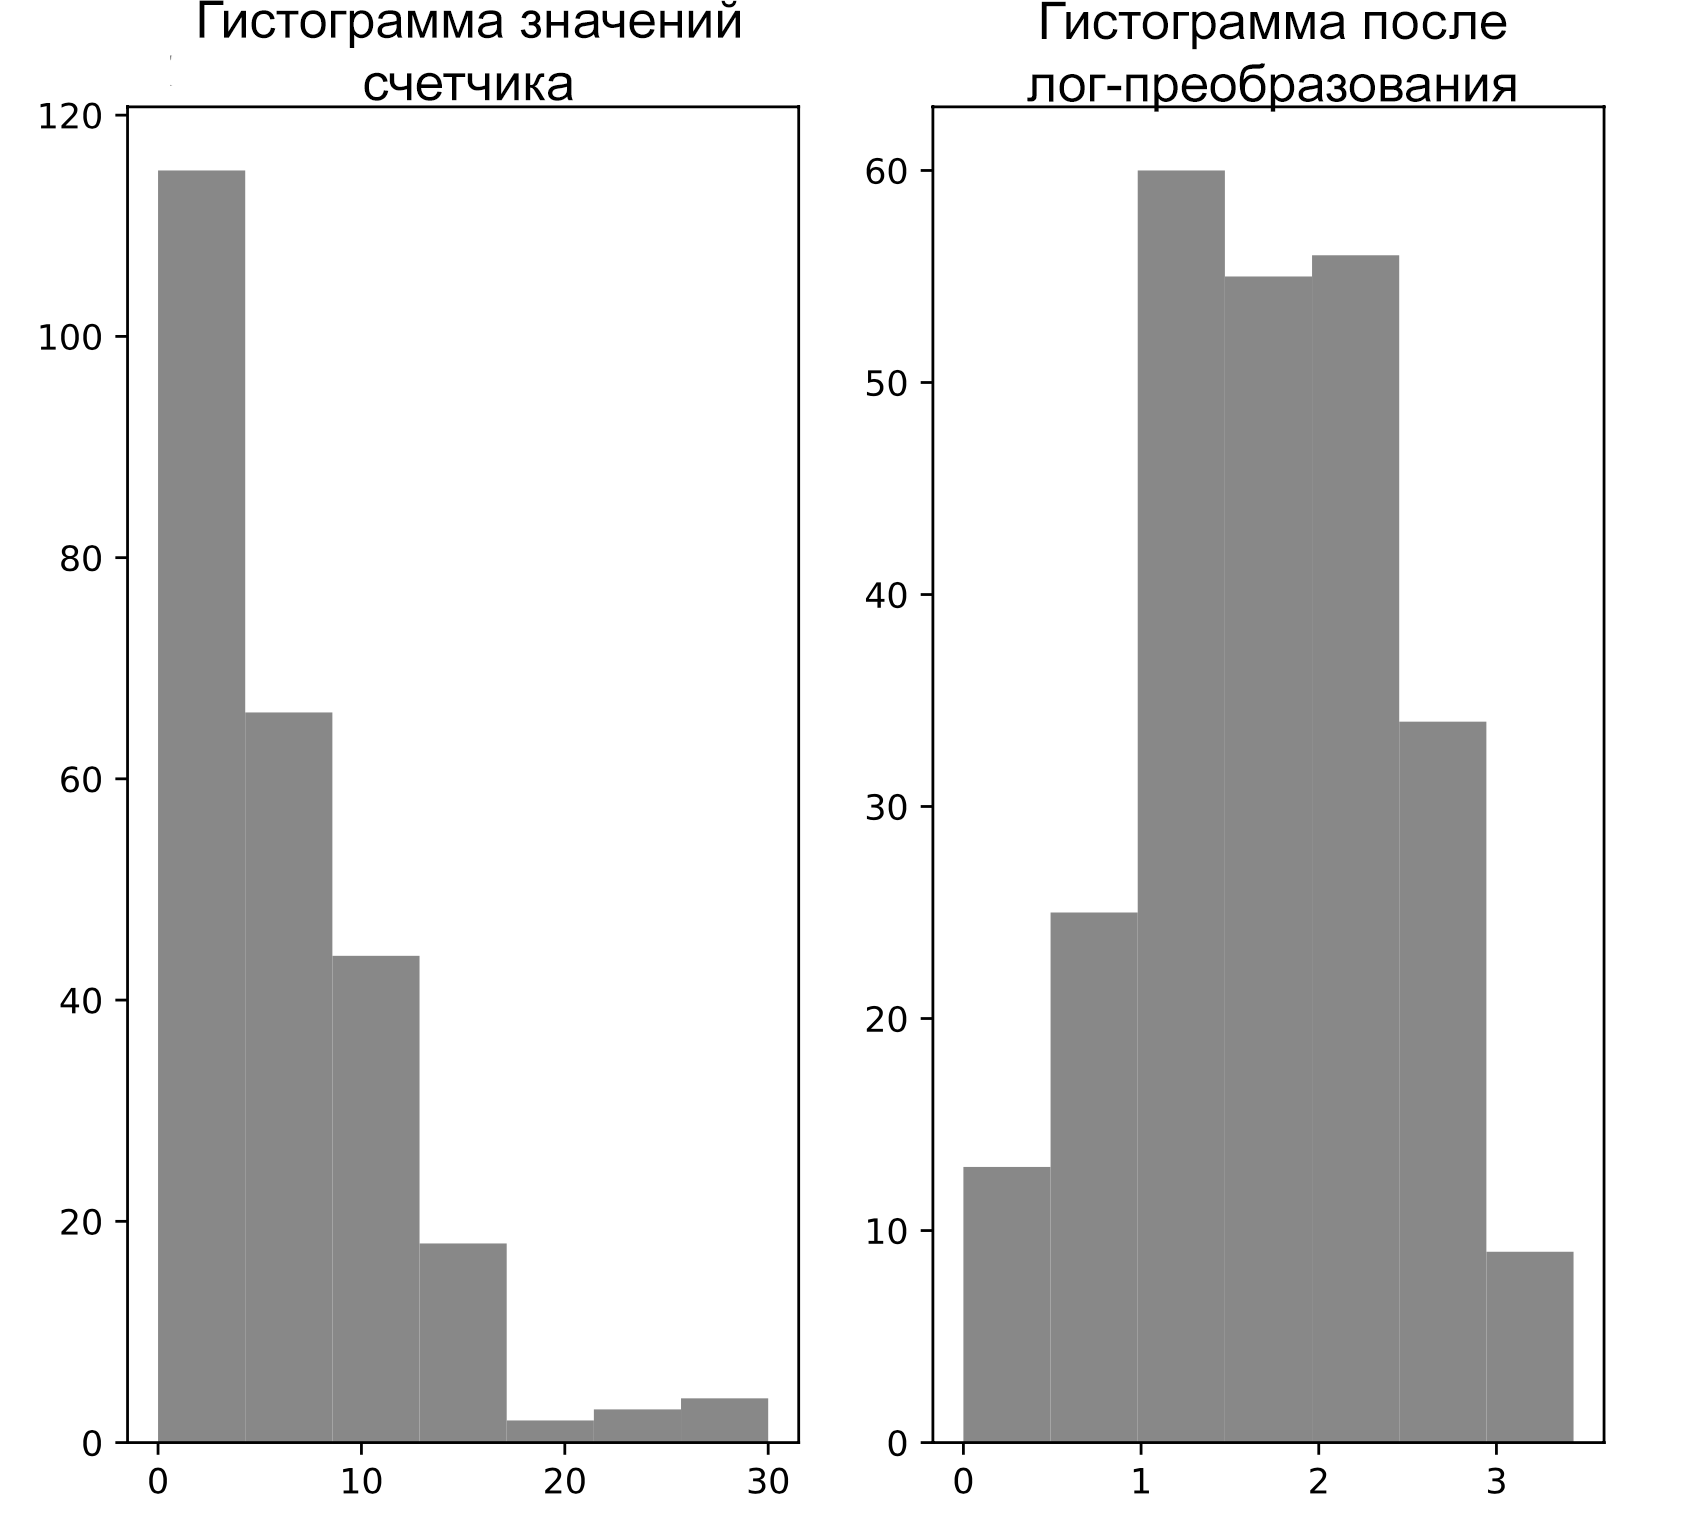
\includegraphics[width=0.45\linewidth]{images/log_hist}
  \caption{Логарифмическое преобразование значений счетчика}
  \label{fig:log_hist}
\end{figure}

По своей природе, целевая переменная в задаче регрессии является счетчиком событий. Исследовав распределение целевой переменной было выяснено, что она имеет распределение Пуассона \cite{pois_handbook}. Исходя из этого было решено предсказывать не количество $n$ событий, а величину $n' = log(1+n)$, восстанавливая затем $n$. Основная мотивация заключается в предположении, что логарифм величины распределенной по закону Пуассона моделировать легче как простыми моделями, такими как линейная регрессия, так и более сложными методами машинного обучения. В таком случае линейная модель регрессии будет называться "Пуассоновской регрессией".

В терминах решаемой задачи, обозначим истинное (прогнозируемое) значение целевой переменной как $y$, а прогноз модели, представляющий из себя логарифм счетчика, как $y'$.

Поскольку оценка моделью значения $y'$ представляет из себя $\mu = \mathbb{E}[\log(y+1)]$, корректное восстановление значения оригинальной целевой переменной $\mathbb{E}[y]$ можно произвести следующим образом: \cite{lognormal}:
$$\mathbb{E}[y]=e^{{\mu + \frac{\sigma ^{2}}{2}}} - 1,$$
где $\sigma$ это стандартное отклонение $y'$. Оценить значение $\sigma$ можно как среднеквадратичную ошибку, посчитанную на отложенной выборке.

Пример значений целевой переменной до и после применения логарифмического преобразования изображен на Рис. \ref{fig:log_hist}

